\subsection{Plane conics and conic surfaces}

\subsubsection{The question of degeneracy}

A plane conic is a algebraic variety $\V(g)$ given by a quadratic form $g \in k[x_0,x_1,x_2]$. One might ask the question whether the conic is a union of two lines (in which case the conic is called \emph{degenerate}), or in algebraic terms, whether $g$ factors into two linear forms or whether it is irreducible.
Let's turn our attention the an easier question: When is a conic singular?

Assume that the characteristic of our base field $k$ is not 2, then the conic can be written, for appropriate coefficients $a,b,c,d,e,f \in k$ as:
\begin{equation}
g = ax_0^2 + bx_0x_1 + cx_1^2 + dx_0x_2 + ex_1x_2 + fx_2^2
\end{equation}
The singular points are given by the system of equations
\begin{equation}
\del_{x_0} g = \del_{x_1} g = \del_{x_2} g = 0
\end{equation}
which written out in matrix notation, amounts to
\begin{align}
\underset{=:M}{\underbrace{
\begin{pmatrix}
2a & b & d \\
b & 2c & e \\
d & e & 2f
\end{pmatrix}
}}
\begin{pmatrix}
x_0 \\ x_1 \\ x_2
\end{pmatrix}
= 0
\end{align}
We call the matrix $M$.
A singular point $[s_0:s_1:s_2] \in \proj^2_k$ would of course be a non-zero solution of above equation and as such can only exist precisely if the determinant of $M$ vanishes.
So far we have obtained

\begin{corollary}
Let $k$ be a field of characteristic not 2 and $g =  ax_0^2 + bx_0x_1 + cx_1^2 + dx_0x_2 + ex_1x_2 + fx_2^2
\in k[x_0,x_1,x_2]$ be a quadratic form. The conic $\V(g) \subset \proj^2_k$ is singular if and only if
\begin{equation}
\frac 12
\det
\begin{pmatrix}
2a & b & d \\
b & 2c & e \\
d & e & 2f
\end{pmatrix}
= 4acf + bde - ae^2 - cd^2 - fb^2
\end{equation}
\end{corollary}

Incidentally this statement holds true for characteristic 2 as well, even though we need to approach the proof a little differently.
At this point I remind the reader that addition and subtraction are the same in characteristic 2, in the sense that negation operation is just the identity, which will simplify the calculations a little.
The corollary then translates to $g$ having a singular point if and only if $bde +ae^2 + cd^2 +fb^2 = 0$.
The set of singular points is by definition the intersection of $V = \V(\del_{x_0}g,\del_{x_1}g,\del_{x_2}g)$ and $\V(g)$, so let's calculate the points in the first variety: Assuming that not all coefficients $b,d,e$ vanish, the only point on $V$ is $[e:d:b]$, as can be seen by Gaussian elimination where we distinguish the cases of $0,1$ or $2$ of the coefficients $b,d,e$ vanishing.
This point $[e:d:b]$ lies on $\V(g)$ iff $0 = g(e,d,b) = ae^2 + bde + cd^2 + dbe + ebd + fb^2 = bde + ae^2 + cd^2 + fb^2$ as desired.
If all of $b,d,e$ vanish, then $V$ is the whole space and every point of $\V(g)$ is singular ($\V(g) = \V((\sqrt{a}x_0 + \sqrt{c}x_1 + \sqrt{f}x_2)^2)$ being a doubled line) and also $bde + ae^2 + cd^2 + fb^2 = 0$. We have proven:

\begin{corollary} \label{corollarySingularConic}
Let $k$ be a field of any characteristic and $g = ax_0^2 + bx_0x_1 + cx_1^2 + dx_0x_2 + ex_1x_2 + fx_2^2
 \in k[x_0,x_1,x_2]$ be a quadratic form. The conic $\V(g) \subset \proj^2_k$ is singular if and only if $4acf + bde - ae^2 - cd^2 - b^2f = 0$.
\end{corollary}


Returning to our initial question we want to establish the fact that the conic given by the quadratic form $g$ is irreducible if and only if it is nonsingular.
For that assume reducibility, that is $g = h_1h_2$ for 1-forms $h_1$ and $h_2$.
We can apply the following lemma
\begin{lemma} \label{lemmaSingularIntersect}
Let $\V(I),\V(J)$ be two varieties. Then the union of $\V(IJ)$ is singular at their intersection $\V(I,J)$.
\end{lemma}
\begin{proof}
Let $f\in I, g\in J$, $P\in \V(I,J)$. We get $(fg)^{(1)}(P) = f(P)g^{(1)}(P) + g(P)f^{(1)}(P) = 0$, hence the tangent space at $P$ is the whole space.
\end{proof}
It says that the intersection of the two lines $\V(h_1)$ and $\V(h_2)$ (and we've seen that lines in $\proj^2_k$ do indeed intersect) is a singular point of our conic.

The converse can be seen as follows. Let $P=[p_0:p_1:p_2]$ be a singularity and $P'=[p'_0:p'_1:p'_2]$ is any other point on the conic (for instance any intersection point of $\V(g) \cap \V(x_i)$, $i$ such that $p_i \neq 0$).
For $g$ to be singular at $P$ means in particular that $g^{(1)}(P,P') = \sum_{i=0}^2 \del_{x_i}g(P)p'_i = 0$ using proposition \ref{propositionTaylor}.
By corollary \ref{corollaryTaylorForQuadricAndCubic}, we can expand $g(\lambda P + \mu P') = \lambda^2 g(P) + \lambda\mu g^{(1)}(P;P') + \mu^2 g(P')= 0$.
Hence $g$ vanishes on the line $\overline{P,P'}$ and Hilbert's Nullstellensatz implies that the conic is a union of two lines.

\begin{theorem}
Let $k$ be a field and $\V(g) \subset \proj^2_k$ a conic given by a quadratic form $g = ax_0^2 + bx_0x_1 + cx_1^2 + dx_0x_2 + ex_1x_2 + fx_2^2$.
Then the following are equivalent:
\begin{enumerate}
\item The conic is degenerate.
\item The quadratic form $g$ factors into two linear forms, $g=h_1h_2$.
\item The conic is singular.
\item $4acf + bde - ce^2 - ad^2 - b^2f = 0$
\end{enumerate}
\end{theorem}


\begin{remark}
Otto Hesse has shown that over $k=\complex$ a curve $\V(g)$ decomposes into lines iff the Hessian curve $\V(\det(\del_{x_i}\del_{x_j}h))$ lies in $\V(g)$ (\cite[p.289]{brieskorn2012plane}), however we've seen that this result does not hold over arbitrary fields.
The equation of the Hessian curve in case of the conic considered in this section is precisely $2(4acf + bde - ce^2 - ad^2 - b^2f) = 0$.
\end{remark}


\subsubsection{The two rulings of a nonsingular quadric surface}


It is now time to profit from the previous meditations about singularities.
Let $Q \subset \proj^3_k$ be a nonsingular quadric surface.
We will see that it does not make sense to count the lines on this surface, but let's find some first.
Surely $Q$ will not contain any plane, as this would mean (appealing to the Nullstellensatz) that $Q$ is the union of two planes.
Furthermore these planes intersect at least in a line, so by lemma \ref{lemmaSingularIntersect} the quadric surface would be singular.
As a first step, choose a point $P \in Q$.
Because $Q$ does not contain planes, the tangent space intersects $Q$ in a conic curve.
This curve is singular at $P$ by lemma \ref{lemmaIntersectionWithTangent}, therefore it is the union of two lines $L_1,L_2$.

Each $L_i$ gives a family of lines as follows: For a point $P'$ on $L_i$, we may intersect again $Q$ with $T_{P'}Q$.
Here too we obtain the union of two lines, one of which being $L_i$, the other line we call $L_i(P')$.
By this definition $L_1(P) = L_2$ and $L_2(P) = L_1$.
We say that the family $\mathcal F(L_i) := \mkset{ L_i(P') }{P' \in L_i}$ is the \emph{family generated by $L_i$}.

In fact, these are all the lines on $Q$, which is obvious from the following consideration.
Let $Z$ be any line on $Q$ which is neither $L_1$ nor $L_2$, then it intersects the plane $T_P(Q)$ in one point (corollary \ref{corollarySimpleIntersect}).
This point lies precisely on one of the two $L_i$ (suppose that was not the case, then $P \in Z \subset Q \implies Z = T_P(Z) \subset T_P(Q) \implies Z=L_1 \text{ or } Z=L_2$) so $Z = L_i(T_P(Q)\cap Z)$.
Conversely note, that we have chosen $P$ arbitrarily, so any point of $Q$ is the intersection of two lines $M_1,M_2$ on $Q$ and each of the two lines belong to the family generated by $L_1$ or $L_2$.
It, however, cannot occur that both lines belong to the same family, say parametrised by $L_1$. In that case, $M_1,M_2,L_1$ would lie on the same tangent plane, but $Q$ intersects a tangent plane in just two lines!
We can conclude therefore:
\begin{proposition}
There are two families $\mathcal F(L_1), \mathcal F(L_2)$ of lines on $Q$ and each line on $Q$ belongs to just one family.
The lines in each family are disjoint and as set the union of any one family covers all of $Q$.
\end{proposition}
A little bit more can be said.
Consider a line $L' \in \mathcal F(L_1)$.
Because $L_1 \in \mathcal F(L')$ and $L_1 \in \mathcal F(L_2)$, the family generated by $L'$ must be $\mathcal F(L_2)$ by previous proposition, but this just means that $L'$ intersects all the lines in $\mathcal F(L_2)$!
Hence we deduced
\begin{corollary} \label{corollaryMutualIntersect}
Any line in $\mathcal F(L_1)$ intersects any other line in $\mathcal F(L_2)$.
\end{corollary}

\begin{figure}
\center
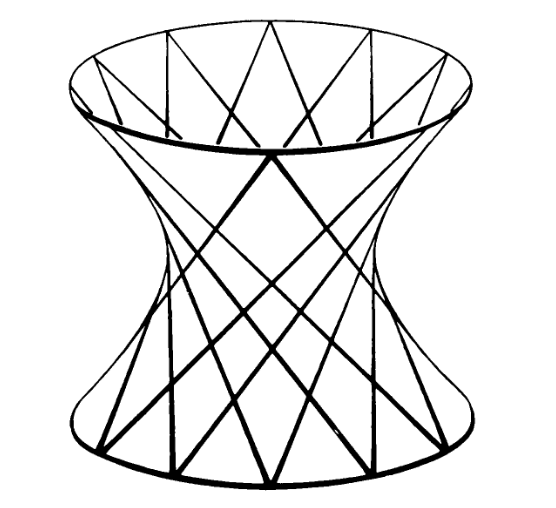
\includegraphics[width=.4\textwidth]{img/ruledsurface-hilbert.png}
\caption{An illustration of the rulings on the quadric surface `Anschauliche Geometrie' by Hilbert and Cohn-Vossen \cite[figure 17]{cohn1990geometry}}
\end{figure}

\begin{remark}
Over an algebraically closed field, a line has infinitely many points, so one cannot hope for the number of lines on a quadric to be finite.
\end{remark}

\begin{remark}
The nonsingular quadric surface $\V(x_0x_3 - x_1x_2)$ is the image of the \emph{Segre map} $\sigma : \begin{cases} \proj^1_k \times \proj^1_k \to& \proj^3_k,  \\ ([x:y],[z:t]) \mapsto& [xz:xt:yz:yt] \end{cases}$.
In this case one can see the ruling easily: The images of
$\sigma(P;\textemdash) : \proj^1_k \to \proj^3_k$ give one family of lines, where $P$ ranges over $\proj^1_k$.
\end{remark}


\begin{lemma} \label{lemmaThreeLines}
Three disjoint lines in $\proj^3_k$ lie on a quadric surface.
Such a quadric surface is necessarily irreducible.
\end{lemma}
\begin{proof}
Let's show irreducibility first.
If three disjoint lines lie on a quadric surface, then this surface cannot be the union of two planes, as two lines on a plane would intersect.
On the existence of the quadric surface:
We are given three disjoint lines with ideals $(h_1,h_2), (h_3,h_4), (h_5,h_6)$, the $h_i$ being linear forms, and want to find a quadratic form $q \in k[x_0,..x_3]$, such that $(h_1,h_2) \cap (h_3,h_4) \cap (h_5,h_6) \supset (q)$ (meaning that the union of the lines contains $\V(q)$).
It suffices to find linear forms $\lambda,\lambda',\mu,\mu',\nu,\nu'$ such that
$\lambda h_1 + \lambda' h_2 = \mu h_3 + \mu' h_4 = \nu h_5 + \nu' h_6 =: q$.
Solving for the linear forms means solving a homogeneous system of linear equations in $6\cdot 4= 24$ variables and $3\binom{4}{2} = 18$ equations, which ensures the existence of $q \neq 0$.
\end{proof}

The following lemma is due to Miles Reid and will be useful to prove the main theorem.
\begin{lemma}
Let $L_1,L_2,L_3,L_4$ be disjoint lines in $\proj^3_k$.
A \emph{transversal} of these lines is a line intersecting all four.
One of the following holds
\begin{enumerate}
\item The $L_i$ line on a irreducible quadric surface $Q$ and there are infinitely many common transversals.
\item No quadric surface contains all the $L_i$. Then there are either one or two common transversals.
\end{enumerate}
\paragraph{Case 1:} Assume there is a quadric containing all lines, necessarily irreducible as seen in the previous lemma.
Then $\mathcal F(L_1)$ is an infinite family of common transversals.
\paragraph{Case 2:} Now assume that there is no quadric containing all four lines.
However by lemma \label{lemmaThreeLines} there exists a quadric surface $Q$ containing the first three lines $L_1,L_2,L_3$.
What can we say about the common transversal of these three?
As $L_1,L_2,L_3$ lie in $Q$, the transversal intersects $Q$ in three distinct points, so by proposition \ref{propositionDegreeOfSurface} it lies on $Q$ already.
A common traversal of all four $L_1,L_2,L_3,L_4$ must therefore lie on $Q$.
By the same proposition \ref{propositionDegreeOfSurface} the line $L_4$ intersects $Q$ in one or two points.
Through each intersection point go 2 lines, but one of them generates the family containing $L_1,L_2,L_3$, so only the other line is a common transversal.
This shows that we have one or two common transversals.
\end{lemma}
